
\begin{questions}

% 1.1  % % % % % % % % % % % % % % % % % % % % %
% \setcounter{question}{1}
\question{
Considere o triângulo no plano definido pelos vértices $a = (1, 1)$, $b = (3, 2)$ e $c = (0, 4)$. Determine o seu ortocentro $h$ (encontro das alturas relativas a seus lados), o seu baricentro $g$ (encontro de suas medianas) e o seu circuncentro $k$ (encontro das mediatrizes relativas aos seus lados). Verifique que estes pontos pertencem a uma mesma reta: a \textit{Reta de Euler}.
}
\begin{solution}

  \begin{minipage}{.5\textwidth}
    \begin{align*}
        & \textcolor{red}{h = (9/7,10/7)}, \\
        & \textcolor{blue}{g = (4/3, 7/3)}, \\
        & \textcolor{green!50!black}{k = (19/14,39/14)}.
    \end{align*}
  \end{minipage}%
  \begin{minipage}{.5\textwidth}
    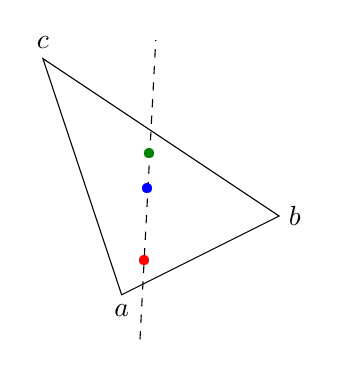
\begin{tikzpicture}
        \draw (1,1) node[anchor=north]{$a$}
            -- (3,2) node[anchor=west]{$b$}
            -- (0,4) node[anchor=south]{$c$}
            -- cycle;
        \draw [dashed] (4/3-0.1,7/3-19*0.1) -- (4/3+0.1,7/3+19*0.1);
        \node [red] at (9/7,10/7) {\textbullet};
        \node [blue] at (4/3,7/3) {\textbullet};
        \node [green!50!black] at (19/14,39/14) {\textbullet};
    \end{tikzpicture}
  \end{minipage}

    Para encontrar $h$, basta resolver o sistema
    \[\begin{cases}
        h_y - c_y = -(1/m_{ab}) (h_x-c_x),\\
        h_y - b_y = -(1/m_{ac}) (h_x-b_x),
    \end{cases}\]
    onde $m_{ab} = (a_y-b_y)/(a_x-b_x)$ e $m_{ac} = (a_y-c_y)/(a_x-c_x)$ são as inclinações das retas $\overline{ab}$ e $\overline{ac}$, respectivamente.
    
    Para encontrar $g$, vide Problema 4.
    
    Para encontrar $k$, basta resolver o sistema
    \[\begin{cases}
        k_y - (a_y+b_y)/2 = -(1/m_{ab}) (k_x-(a_x+b_x)/2),\\
        k_y - (a_y+c_y)/2 = -(1/m_{ac}) (k_x-(a_x+c_x)/2).
    \end{cases}\]
    
    Para mostrar que $h$, $g$ e $k$ são colineares, basta verificar que a seguinte igualdade é verdadeira \vspace{-5mm}
    \begin{align*}
        \frac{h_y - g_y}{h_x - g_x} = \frac{g_y - k_y}{g_x - k_x}.
    \end{align*}
\end{solution}

% 1.2 % % % % % % % % % % % % % % % % % % % % %
% \setcounter{question}{2}
\question{
Considere o vetor $\vec p = (1,2,-1) \in \R^3$. Encontre escalares $a,b,c$ tais que
\[
\vec p = a(1,0,1) + b(0,1,1) + c(1,1,0).
\]
Para qualquer vetor $\vec p$, sempre é possível encontrar escalares que validem a igualdade acima? Justifique em caso afirmativo ou encontre um contra-exemplo.
}

\begin{solution}
    Os vetores são linearmente independentes. Portanto, a solução existe e é única para qualquer vetor do $\R^3$. Para o caso de $\vec p$, temos que $a=-1$, $b=0$, $c=2$.
\end{solution}

% 1.3 % % % % % % % % % % % % % % % % % % % % %
% \setcounter{question}{2}
\question{
    Encontre dois vetores perpendiculares entre si que são ortogonais a $(1,1,0)$.
}

\begin{solution}
    Dois possíveis vetores são $(0,0,1)$ e $(1,-1,0)$.
\end{solution}

% 1.4 % % % % % % % % % % % % % % % % % % % % %
% \setcounter{question}{2}
\question{
    Calcule a distância entre as retas $\vec r = (1,0,0) + \big[(1,2,0)\big]$ e $\vec s = (2,3,1) + \big[(1,0,1)\big]$.
}

\begin{solution}
    Sejam as retas $\vec r(t) = \vec r_0 + t\,\vec r_d$, $t\in\R$ e $\vec s(w) = \vec s_0 + w\,\vec r_d$, $w\in\R$. Sabemos que a distância entre as retas é calculada através do segmento de reta perpendicular à ambas. Podemos encontrar um vetor perpendicular $\vec n$ às duas retas fazendo o produto vetorial entre os vetores diretores, ou seja, $\vec n = \vec r_d \times \vec s_d$ e o unitário $\hat n = \vec n/|\vec n|$.
    
    Em seguida, basta encontrarmos o parâmetro $\lambda\in\R$ que satisfaz a seguinte equação
    \begin{equation*}
        \vec r(t) + \lambda \, \hat n = \vec s(w)
    \end{equation*}
    para algum valor de $t,w\in\R$.
    Podemos aplicar o produto interno com $\vec n$ em ambos lados da equação para obter
    \vspace{-3mm}
    \begin{align*}
        (\vec r_0 + t\,\vec r_d) \cdot \hat n + \lambda = (\vec s_0 + w\,\vec s_d)\cdot \hat n.
    \end{align*}
    Lembrando que $\hat n$ é ortogonal à $\vec r_d$ e $\vec s_d$, temos que
    \begin{align*}
        \lambda = (\vec s_0 - \vec r_0) \cdot \hat n.
    \end{align*}
    Dessa forma, a distância entre as retas $\vec r$ e $\vec s$ é dada por \vspace{-2mm}
    \begin{align*}
        \boxed{d(\vec r,\vec s) = \left| \frac{(\vec r_0 - \vec s_0) \cdot (\vec r_d \times \vec s_d)}{|\vec r_d \times \vec s_d|} \right|}.
    \end{align*}
    Aplicando os valores do enunciado, temos que $d(\vec r,\vec s) = 1$.
\end{solution}

% 1.6 % % % % % % % % % % % % % % % % % % % % %
\setcounter{question}{5}
\question{
Determine uma equação para o plano $\pi$ que passa por $(1,2,1)$ e tem vetor normal $(0,1,1)$. Calcule a distância deste plano até a origem.
}
\begin{solution}
    Seja $\vec r_0 = (1,2,1)$ e $\vec n = (0,1,1)$. Se $r\in\pi$, então \vspace{-2mm}
    \[\vec n \cdot (\vec r - \vec r_0) = 0.\]
    Logo, \vspace{-3mm}
    \[\pi = \left\{(x,y,z)\in\R^3 \mid y + z = 3 \right\}.\]
\end{solution}


% 1.8  % % % % % % % % % % % % % % % % % % % % %
\setcounter{question}{7}
\question{
Se $\vec r = (x,y)$, $\vec r_1 = (x_1,y_1)$ e $\vec r_2 = (x_2,y_2)$, descreva o conjunto dos pontos $(x,y)$ tais que
\[
    |\vec r - \vec r_1| + |\vec r - \vec r_2| = k,
\]
para alguma constante $k > |\vec r_1 - \vec r_2|$. 
}

\begin{solution}
    Todos os pontos de uma elipse têm a propriedade da soma da distância deles com os focos ser constante. Logo, trata-se de uma elipse com focos em $\vec r_1$ e $\vec r_2$.
\end{solution}

% 1.9 % % % % % % % % % % % % % % % % % % % % %
% \setcounter{question}{5}
\question{
Um tetraedro $OPQR$ tem como arestas os vetores $\overrightarrow{OP} = 2\hat \imath+ 4\hat \jmath $, $\overrightarrow{OQ} = 2\hat \imath- \hat \jmath+ 3\hat k$ e $\overrightarrow{OR} = 4 \hat \imath- 2\hat \jmath+ 5\hat k$. Mostre que $\overrightarrow{OP}$ é ortogonal ao plano $OQR$. Use essa informação para calcular o volume do tetraedro.
}

\begin{solution}
    O vetor $\overrightarrow{OP}$ é ortogonal ao plano $OQR$, pois $\overrightarrow{OP} \cdot \overrightarrow{OQ} = 0$ e $\overrightarrow{OP} \cdot \overrightarrow{OR} = 0$.
    
    O volume do tetraedro é dado por \vspace{-3mm}
    \begin{align*}
        V_{OPQR} = \left| \frac{1}{6} \left(\overrightarrow{OQ} \times \overrightarrow{OR}\right) \cdot \overrightarrow{OP} \right|
            = \frac{5}{3}.
    \end{align*}
\end{solution}

% 7.12 % % % % % % % % % % % % % % % % % % % % %
% \setcounter{question}{11}
\question{
Calcule a área do triângulo com vértices $A = (1,4,6)$, $B = (-2,5,-1)$ e $C = (1,-1,1)$. Use o Problema 8.
}
\begin{solution}
\begin{align*}
    A_{ABC} = \frac{|\overrightarrow{AB}\times \overrightarrow{AC}|}{2}
        = \frac{1}{2} |(-40,-15,15)| = \frac{5}{2} \sqrt{82}.
\end{align*}
\end{solution}

\end{questions}
